\chapter{Neural network}\label{nn}

\section{Neural network architecture}

Given the nature of the data, we decided to use a neural network to predict the
changes in the body shape. Since the data is temporal, we need to use a neural
network architecture that can handle temporal data.

There are different neural network architectures that work well with temporal
data. Recurrent neural networks are a type of neural networks that feed the
output of the previous step as input to the next step. This allows them to
remember information from previous steps, which is useful for time series.
However, they can `forget' information from the beginning of the sequence,
which is a problem known as vanishing gradients. There are some variations of
recurrent neural networks that try to solve this problem, such as \gls{lstm}
and \gls{gru}.

Transformer networks are a relatively new type of neural network that has been
used with great success in natural language processing. They are based on
attention mechanisms, which allow them to focus on specific parts of the input
sequence. This makes them very useful for time series, since they can focus on
the most relevant parts of the sequence. The big disadvantage of transformer
networks for this application is that they require large amounts of training
data\todo[]{citation needed}, which is not available in this case.

We ended up using an neural network architecture that uses an \gls{lstm}.

\section{Training}

\subsection{Variability in the dates of the sessions}

The dataset's sessions are not uniformly spaced in time, varying from a few
days to several months apart. To mitigate this issue, we:

Calculated a variable representing the number of days until the next session.

Modified the neural network to predict the daily change in variables, instead
of predicting the variables for the following session.

We implemented a residual connection to the neural network, enabling it to
predict the change in variables from one session to the next. Then, we
multiplied this change by the number of days until the next session and added
it to the previous session to calculate the predicted values for the next
session. This approach assumes a linear change between sessions—an
approximation suited to our purpose. We augmented the data by randomly removing
intermediate sessions and recalculating the number of days until the next
session.

\section{Neural network architecture}

We used the PyTorch library to implement our custom neural network
architecture.

\begin{figure}
    \centering
    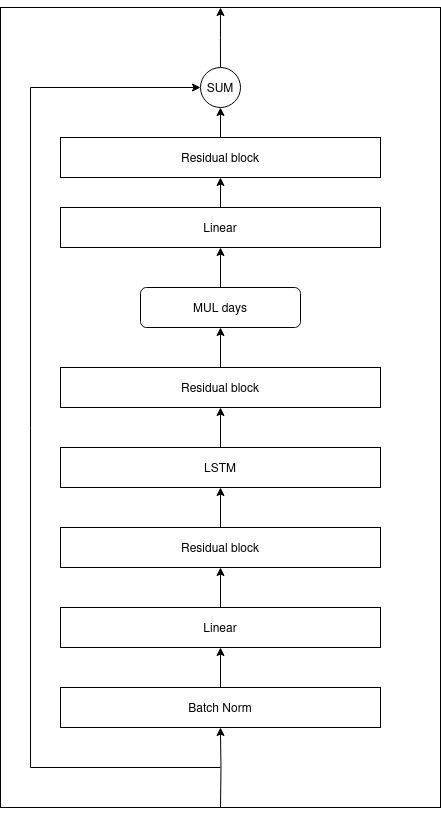
\includegraphics[width=6cm]{files/nn_diagram}
    \caption{Diagram of the neural network architecture}
\end{figure}

This architecture can handle temporal data of varying lengths.

\section{Training}

The neural network inputs a tensor of shape (batch size, max sequence length,
number of features), a tensor of shape (batch size, 1) containing the length of
the current sequence, and a scalar representing the number of days until the
next session. It returns a tensor of shape (batch size, max sequence length,
number of features) containing the predicted values for the next session.

\begin{itemize}
    \item The neural network takes as input:
          \begin{itemize}
              \item A tensor of shape (batch size, max sequence length, number of features).
              \item A tensor of shape (batch size, 1) containing the length of the current
                    sequence.
              \item A scalar representing the number of days until the next session.
          \end{itemize}
    \item The neural network returns:
          \begin{itemize}
              \item A tensor of shape (batch size, max sequence length, number of features) that
                    contains the predicted values for the next session.
          \end{itemize}
\end{itemize}

For features, we concatenate the \gls{smpl} parameters shape ($\beta$) with the
patient's height, weight, and age. We also experimented with using body fat
percentage and muscle mass percentage, but the results were comparable. We used
the AdamW optimizer with a variable learning rate and weight decay, and MSE
loss.

\section{Evaluation}

The mean absolute error (MAE) of the predicted betas served as our evaluation
metric.

\section{Results}

\begin{figure}[h]
    \centering
    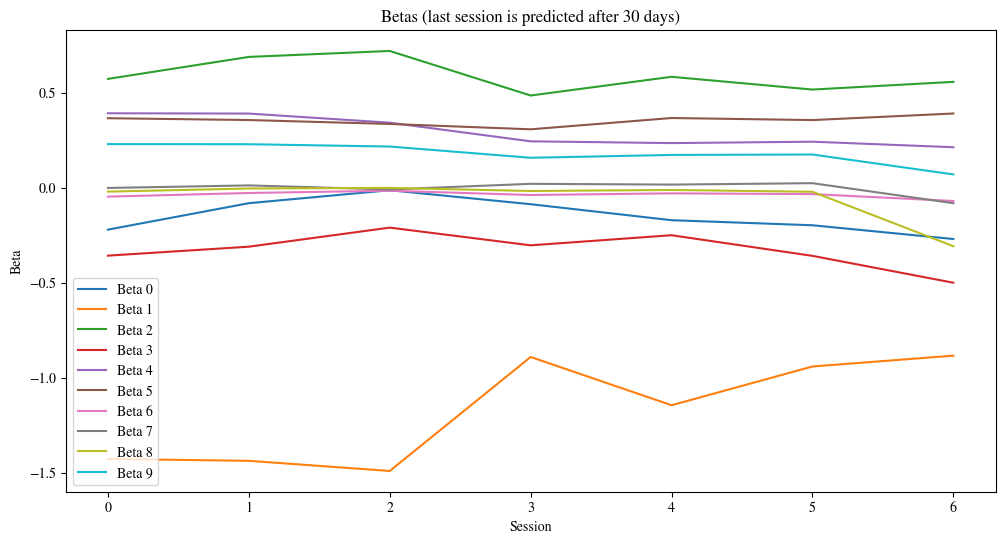
\includegraphics[width=\textwidth]{files/predicted_betas}
    \caption{Change of the shape parameters for a given patient and the neural
        network prediction after 30 days}
\end{figure}